%======================================================================
% fazove_prechody_solution.pdf
%======================================================================
\section{Cvičení: Fázové přechody -- řešení}
\strana{FPsol-1}

\begin{priklad}[Příklad 1$^*$]
Vysoká, nahoře otevřená nádoba je částečně naplněna kapalinou a ochlazena na $-5\,^\circ$C. Při této teplotě látka u dna stuhne až
do výšky $h$ a nad touto úrovní zůstane v kapalné fázi. Pokud teplotu dále snížíme na $-5.2\,^\circ$C, rozhraní pevná fáze-kapalina se
zvedne o $\Delta h = 40$\,cm. Latentní teplo tání je $l = 2$\,cal/g a hustota kapalné fáze je $1$\,g/cm$^3$. Jaká je hustota pevné fáze?
Teplotní roztažnost obou fází zanedbejte.
\end{priklad}

\begin{center}
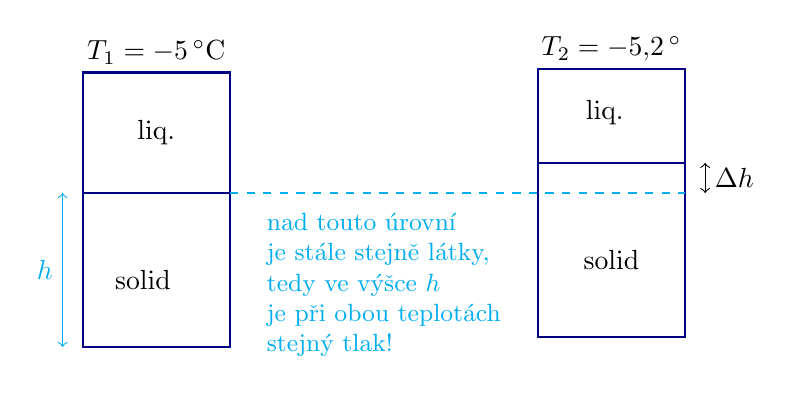
\begin{tikzpicture}[scale=0.85]
  % levá nádoba
  \draw[NavyBlue,thick] (0,0) rectangle (2.2,4.1);
  \draw[NavyBlue,thick] (0,2.3) -- (2.2,2.3);
  \node at (1.1,4.4) {$T_1 = -5\,^\circ$C};
  \node at (1.1,3.2) {liq.};
  \node at (0.9,1.0) {solid};
  \draw[<->,cyan] (-0.3,0) -- (-0.3,2.3) node[midway,left] {$h$};
  % pravá nádoba
  \draw[NavyBlue,thick] (6.8,0.15) rectangle (9,4.15);
  \draw[NavyBlue,thick] (6.8,2.75) -- (9,2.75);
  \node at (7.9,4.45) {$T_2 = -5{,}2\,^\circ$};
  \node at (7.8,3.5) {liq.};
  \node at (7.9,1.3) {solid};
  \draw[<->] (9.3,2.3) -- (9.3,2.75) node[midway,right] {$\Delta h$};
  % čárkovaná úroveň
  \draw[dashed,cyan] (2.2,2.3) -- (9,2.3);
  \node[cyan,align=left,font=\small,anchor=north] at (4.5,2.15) {nad touto úrovní\\ je stále stejně látky,\\ tedy ve výšce $h$\\ je při obou teplotách\\ stejný tlak!};
\end{tikzpicture}
\end{center}

\begin{itemize}
  \item změna teploty $T_1\to T_2$ vede k poklesu tlaku koexistence pevné a kapalné fáze o $\Delta p = g\rho_l\Delta h$
        (výška sloupce kapaliny nad rozhraním se sníží o $\Delta h$)
  \item Clapeyron: \quad $\dfrac{\dd p}{\dd T} = \dfrac{l}{T\Delta v}$ \qquad
        $\Delta v = v_l - v_s = \dfrac{1}{\rho_l} - \dfrac{1}{\rho_s}$ \qquad
        \\ \hspace*{2.2cm}\textcolor{Red}{$\nabla$ $l > 0 \Leftrightarrow \Delta S > 0$ \ $\Uparrow$ solid $\to$ liquid} \\
        \hspace*{2.2cm}$\Downarrow$ \\
        \hspace*{1.6cm}$\Delta p \sim \dfrac{l}{T\Delta v}\,\Delta T$
\end{itemize}
\[
  \Rightarrow\quad g\rho_l\Delta h = \frac{l}{T_1\big(\frac{1}{\rho_l} - \frac{1}{\rho_s}\big)}\,\Delta T
  \qquad\Rightarrow\quad \rho_s =
\]

\begin{priklad}[Příklad 4$^*$]
V blízkosti trojného bodu NH$_3$ je tlak nasycené páry na kapalnou fází popsán rovnicí ($p$ v Pa)
\[
  \log p = 24{,}38 - \frac{3063}{T} \qquad (1)
\]
a nad pevnou fází rovnicí
\[
  \log p = 27{,}92 - \frac{3754}{T}. \qquad (2)
\]
Najděte trojný bod $(T,\,p)$. Jaká jsou latentní tepla sublimace a varu? Jaké je latentní teplo tání v blízkosti trojného bodu?
\end{priklad}

1 \& 2 jsou zjevně křivky koexistence $g\leftrightarrow l$ \& $g\leftrightarrow s$ \\
$\Rightarrow$ trojný bod je dán \quad $(1) = (2)$

\[
  \frac{\dd p}{\dd T} = \frac{l}{T\Delta v} \ \Rightarrow\ l = T\Delta v\,\frac{\dd p}{\dd T}
\]
\& v obou případech lze aproximovat (viz Clausius-Clapeyron) \quad $\Delta v \approx v_g = \dfrac{RT}{p}$

%----------------------------------------------------------------------
\strana{FPsol-2}
\[
  \Rightarrow\quad \vzorec{l = \frac{RT^2}{p}\,\frac{\dd p}{\dd T}}\ ,
  \qquad\text{kde } \frac{\dd p}{\dd T} \text{ je derivace (1) pro } l_{\text{var}} \text{ a (2) pro } l_{\text{sub}}
\]
\begin{itemize}
  \item $l_{\text{tání}}$ odhadneme tak, že předpokládáme, že \\
        \quad \uv{tání $=$ sublimace $\to$ kondenzace} \quad $\Rightarrow$ \quad $l_{\text{tání}} \approx l_{\text{sub}} - l_{\text{var}}$
  \item ve $\forall$ vztazích pro num.\ výsledek dosazuji $T, p =$ trojný bod určený v prvním úkolu
\end{itemize}

\begin{priklad}[Příklad 2$^*$ \ {[Callen 9.7-1,2]}]
Uvažujme fázový diagram dvousložkového systému. Pro konkrétní tlak je v $(T, c_1)$ reprezentaci oblast koexistence plynné a kapalné
fáze ohraničena funkcemi
\[
  T = T_0 - (T_0 - T_1)c_1^2 \quad (1) \qquad\text{a}\qquad T = T_0 - (T_0 - T_1)c_1(2 - c_1), \quad (2)
\]
kde $c_1$ je koncentrace \uv{první} složky. Kapalina se nachází hluboko pod teplotou varu a počáteční koncentrace je $c_1 = 1/2$.
\begin{enumerate}[label=\alph*)]
  \item Směs uvedeme za konstantního tlaku k varu. Jaká bude koncentrace $c_1$ v páře ve chvíli, kdy se směs právě začne vařit?
  \item Je-li $\big(-\frac{dN}{N}\big) > 0$ úbytek látky v kapalném skupenství, ukažte, že
        \[ dc_1 = -\big[(2c_1 - c_1^2)^{1/2} - c_1\big]\Big(-\frac{dN}{N}\Big) \]
        je změna koncentrace první složky v kapalině.
  \item Popište na tomto diagramu celý proces vypařování a vysvětlete, proč nelze v procesu destilace získat ani minimální množství
        čisté složky 1 nebo 2 ani v plynném, ani v kapalném skupenství.
\end{enumerate}
\end{priklad}

\begin{center}
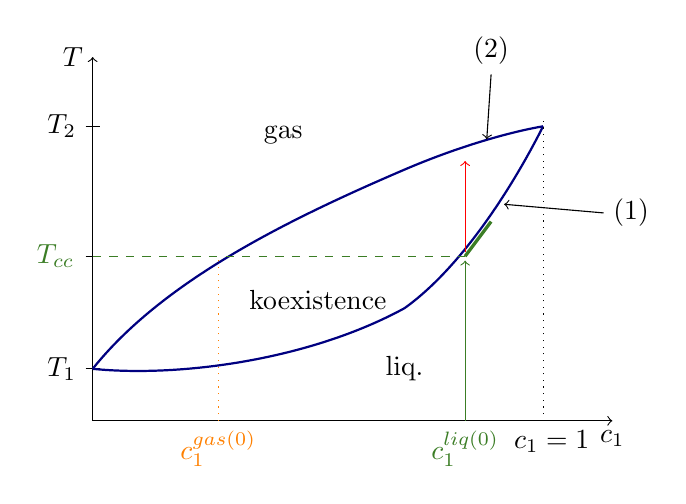
\begin{tikzpicture}[scale=1.1]
  \draw[->] (0,0) -- (6,0) node[below] {$c_1$};
  \draw[->] (0,0) -- (0,4.2) node[left] {$T$};
  % T1, T2
  \draw (-0.08,0.6) -- (0.08,0.6) node[pos=0,left] {$T_1$};
  \draw (-0.08,3.4) -- (0.08,3.4) node[pos=0,left] {$T_2$};
  \draw (-0.08,1.9) -- (0.08,1.9);
  \node[OliveGreen,left] at (-0.1,1.9) {$T_{cc}$};
  % křivka (2) horní -- plyn
  \draw[NavyBlue,thick] (0,0.6) .. controls (0.8,1.6) and (2.2,2.3) .. (3.6,2.9) .. controls (4.3,3.2) and (4.9,3.35) .. (5.2,3.4);
  % křivka (1) dolní -- kapalina
  \draw[NavyBlue,thick] (0,0.6) .. controls (1,0.5) and (2.5,0.7) .. (3.6,1.3) .. controls (4.3,1.8) and (4.9,2.8) .. (5.2,3.4);
  % úsečka koexistence
  \draw[OliveGreen,dashed] (0,1.9) -- (4.3,1.9);
  \draw[orange,dotted] (1.45,0) -- (1.45,1.9);
  \draw[OliveGreen,->] (4.3,0) -- (4.3,1.85);
  \draw[Red,->] (4.3,1.95) -- (4.3,3.0);
  \draw[OliveGreen,very thick] (4.3,1.9) -- (4.6,2.3);
  \draw[dotted] (5.2,0) -- (5.2,3.5);
  \node at (2.2,3.3) {gas};
  \node at (2.6,1.4) {koexistence};
  \node at (3.6,0.6) {liq.};
  \draw[->] (4.6,4.0) node[above] {(2)} -- (4.55,3.25);
  \draw[->] (5.9,2.4) node[right] {(1)} -- (4.75,2.5);
  \node[orange,below] at (1.45,0) {$c_1^{\text{gas}(0)}$};
  \node[OliveGreen,below] at (4.3,0) {$c_1^{\text{liq}(0)}$};
  \node[below] at (5.3,0) {$c_1 = 1$};
\end{tikzpicture}
\end{center}

a) \quad $T_{cc} = (1)\big/_{c_1 = c_1^{\text{liq}(0)}}$ \\
\phantom{a)} \quad\ $\downarrow$ \\
\phantom{a)} \quad $T_{cc} = (2)\big/_{c_1 = c_1^{\text{gas}(0)}}$ \quad $\to$ \quad $c_1^{\text{gas}(0)} =$

c) bylo na přednášce

b) během vypařování se celý systém pohybuje po \textcolor{Red}{vertikále $c_1 = c_1^{\text{liq}(0)}$}, ale kapalná složka
\textcolor{OliveGreen}{sleduje \uv{svoji nadplochu (1)}}. Poměr kapalné vs.\ plynné složky je přitom dán \uv{(horizontálním) pákovým
pravidlem}. Dokončete :-) sami
